%! TEX root = ../../master.tex
\lecture[Convex duality. $\IP$ solving strategies. Integrality of $\LP$s. Totally unimodular matrices. Network matrices.]{Di 10 May 2022}{Convex duality \& integral LPs}
Note that the function isn't smooth, but still we can define a notion for their gradient:
\begin{definition}
    We call the set of possible "derivatives" in a point of a function the \vocab{subdifferential}.
\end{definition}
Let's visualize using previous example, \autoref{fig:prim-dual-cost}.
\begin{figure*} \label{fig:prim-dual-cost}
    \centering
    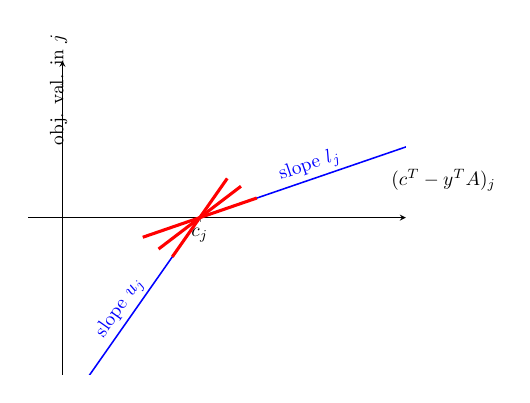
\begin{tikzpicture}[scale=0.7]
        \begin{axis}[
                axis x line=center,
                axis y line=middle,
                xlabel=$(c^T-y^TA)_j$,
                ylabel=obj. val. in $j$,
                ylabel style={sloped, xshift=-15pt, yshift=10pt},
                xlabel style={xshift=50pt, yshift=10pt},
                grid=none,
                ytick={0},
                xtick={2},
                xticklabel={$c_j$},
                xmin=-0.5,
                xmax=5,
                ymin=-4,
                ymax=4,
                % minor tick num=1,
                % axis equal image,
            ]
            \addplot[blue, thick] coordinates {(2,0) (5.33,2)}
            node[pos=0.5, yshift=7pt,sloped]{slope $l_j$}
            ;
            \addplot[blue, thick] coordinates {(0,-5) (2,0)}
            node[pos=0.5, yshift=7pt,sloped]{slope $u_j$}
            ;
            \addplot[red, ultra thick] coordinates {(2.83,0.5) (1.17,-0.5)};
            \addplot[red, ultra thick] coordinates {(2.6,0.8) (1.4,-0.8)};
            \addplot[red, ultra thick] coordinates {(2.4,1) (1.6,-1)};
        \end{axis}
    \end{tikzpicture}
    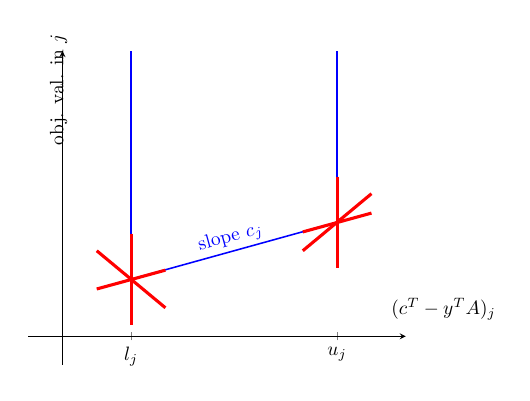
\begin{tikzpicture}[scale=0.7]
        \begin{axis}[
                axis x line=center,
                axis y line=middle,
                xlabel=$(c^T-y^TA)_j$,
                ylabel=obj. val. in $j$,
                ylabel style={sloped, xshift=-20pt,yshift=10pt},
                xlabel style={xshift=50pt, yshift=5pt},
                grid=none,
                ytick={0},
                xtick={1,4},
                xticklabels={$l_j$,$u_j$},
                xmin=-0.5,
                xmax=5,
                ymin=-0.5,
                ymax=5,
                % minor tick num=1,
                % axis equal image,
            ]
            \addplot[blue, thick] coordinates {(1,1) (4,2)}
            node[pos=0.5, yshift=7pt,sloped]{slope $c_j$}
            ;
            \addplot[blue, thick] coordinates {(4,2) (4,5)};
            \addplot[blue, thick] coordinates {(1,1) (1,5)};

            \addplot[red, ultra thick] coordinates {(1,1.8) (1,0.2)};
            \addplot[red, ultra thick] coordinates {(1.5,1.16) (0.5,0.83)};
            \addplot[red, ultra thick] coordinates {(1.5,0.5) (0.5,1.5)};

            \addplot[red, ultra thick] coordinates {(4,2.8) (4,1.2)};
            \addplot[red, ultra thick] coordinates {(4.5,2.16) (3.5,1.83)};
            \addplot[red, ultra thick] coordinates {(4.5,2.5) (3.5,1.5)};
        \end{axis}
    \end{tikzpicture}
    \caption{Exemplary dual and primal cost function in $j$th component with subset of subdifferentials in red}
\end{figure*}
Let's also consider the implications for optimal solutions from complementary slackness:
\begin{itemize}
    \item For $\lambda_j > 0$ follows that $c_j > (y^TA)_j$ ("expensive"), and by CS $x_j=l_j$.
    \item For $\mu_j > 0$ follows that $c_j < (y^TA)_j$ ("cheap"), and by CS $x_j=u_j$.
    \item For $c_j = (y^TA)_j$ ("neutral") follows by CS that $l_j\leq x_j\leq u_j$.
\end{itemize}
\begin{definition}[Kilter diagram]
    We can visualize variable-constraint pairs of complementary slackness with a \vocab{Kilter diagram}.
\end{definition}
\begin{example} Again, using our system, we can draw the primal and dual Kilter diagram:
    \\
    \begin{minipage}{\textwidth}
        % \centering
        \begin{tikzpicture}[scale=0.7]
            \begin{axis}[
                    axis x line=center,
                    axis y line=middle,
                    xlabel=$x_j$,
                    ylabel=$(y^TA)_j$,
                    ylabel style={sloped, xshift=-20pt,yshift=15pt},
                    xlabel style={xshift=50pt, yshift=5pt},
                    grid=none,
                    ytick={2},
                    xtick={1,4},
                    xticklabels={$l_j$,$u_j$},
                    yticklabels={$c_j$},
                    xmin=-0.5,
                    xmax=5,
                    ymin=-0.5,
                    ymax=5,
                    % minor tick num=1,
                    % axis equal image,
                ]
                \addplot[blue, thick] coordinates {(1,2) (4,2)};
                \addplot[blue, thick, dotted] coordinates {(1,0) (1,2)}
                node[pos=0.5, yshift=7pt,sloped]{"expensive"}
                ;
                \addplot[blue, thick, dotted] coordinates {(4,2) (4,5)}
                node[pos=0.5, yshift=7pt,sloped]{"cheap"}
                ;
            \end{axis}
        \end{tikzpicture}
        \begin{tikzpicture}[scale=0.7]
            \begin{axis}[
                    axis x line=center,
                    axis y line=middle,
                    ylabel=$x_j$,
                    xlabel=$(y^TA)_j$,
                    ylabel style={sloped, xshift=-20pt,yshift=10pt},
                    xlabel style={xshift=50pt, yshift=5pt},
                    grid=none,
                    ytick={1,4},
                    xtick={2},
                    yticklabels={$l_j$,$u_j$},
                    xticklabels={$c_j$},
                    xmin=-0.5,
                    xmax=5,
                    ymin=-0.5,
                    ymax=5,
                    % minor tick num=1,
                    % axis equal image,
                ]
                \addplot[blue, thick, dotted] coordinates {(2,1) (2,4)}
                % node[pos=0.5, yshift=7pt,sloped]{slope $c_j$}
                ;
                \addplot[blue, thick] coordinates {(2,1) (0,1)};
                \addplot[blue, thick] coordinates {(2,4) (5,4)};

            \end{axis}
        \end{tikzpicture}
    \end{minipage}
\end{example}
\begin{fact}[Convex duality]
    If term $j$ of the primal objective is $f_j(x_j)$ for convex $f_j$,
    then term $j$ of the dual objective is $-f_j^\bullet(y_j)$, such that
    $y_j$ is the dual of $x_j$.

    We're using $f^\bullet$ as the \vocab{convex conjugate} of $f$, which has the property that
    $(f^\bullet)^\bullet=f$.
\end{fact}
Now, consider some piecewise linear convex function with slopes $m_i$ and breakpoints $b_i$.
\\
\begin{minipage}{\textwidth}
    \centering
    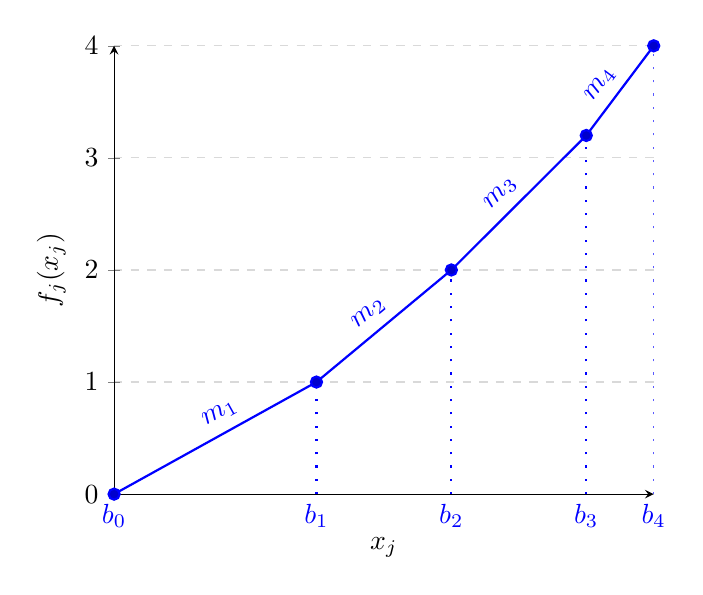
\begin{tikzpicture}
        \begin{axis}[
                axis x line=bottom,
                axis y line=left,
                grid = major,
                grid style={dashed, gray!30},
                % width = 16cm,
                % height = 8cm,
                xmin = 0,
                xmax = 8,
                ymin = 0,
                ymax = 4,
                xlabel = $x_j$,
                ylabel = $f_j(x_j)$,
                xlabel shift = 10,
                xtick = \empty
            ]
            % \addplot[domain=1:8, blue, thick, samples=100]{x < 2 ? 0.5*x : (x < 4 ? x - 1 : (x < 5 ? 11 - 2 *x : 1.5 *x-9))};
            \addplot+[blue,thick] coordinates {
                    (0, 0)
                    (3,1)
                    (5, 2)
                    (7, 3.2)
                    (8, 4)
                }
            node[pos=0.2, yshift=7pt,sloped]{$m_1$}
            node[pos=0.47, yshift=7pt,sloped]{$m_2$}
            node[pos=0.72, yshift=7pt,sloped]{$m_3$}
            node[pos=0.92, yshift=7pt,sloped]{$m_4$}
            ;
            \addplot[ycomb,
                blue,thick,loosely dotted,
                symbolic x coords={a,b,c,d,e,f}
            ] coordinates {
                    (0, 0)
                    (3,1)
                    (5, 2)
                    (7, 3.2)
                    (8, 4)
                };
            \addplot[blue,nodes near coords,
                nodes near coords align=below,
                only marks,
                point meta=explicit symbolic]
            coordinates {
                    (0, 0)[$b_0$]
                    (3,0)[$b_1$]
                    (5, 0)[$b_2$]
                    (7, 0)[$b_3$]
                    (8, 0)[$b_4$]
                };
        \end{axis}
    \end{tikzpicture}
\end{minipage}
We can express values on this function with following LP:
\begin{mini*}{x}{m_1x_{j,1}+m_2x_{j,2}+m_3x_{j,3}+\dots}{}{}
    \addConstraint{0}{\leq x_{j,i} \leq b_i - b_{i-1}, \quad}{i=1,\dots}
    \addConstraint{x_j}{=x_{j,1}+x_{j,2}+x_{j,3}}
\end{mini*}
Note that this forces the $\LP$ to use as much of $x_{j,i}$ as possible before moving to the next component.
\begin{conclusion}
    Piecewise linear convex problems don't need  $\IP$.
\end{conclusion}
\begin{note}
    In fact, $\IP$ is only needed for non-convex/non-concave functions, see \cite[Ch.~14]{network-flows}.
\end{note}


\section{Approaches to $\IP$}
Even though $\IP$ is $\NP$-complete, we still want to solve them as they model many real-world problems.
For certain cases, though, we can use tricks to make calculation easier:
\begin{enumerate}
    \item If the $\IP$ only has integer vertices for all $b$, we can just use $\LP$.
    \item If the $\IP$ only has integer vertices for a single useful $b$, we can at least use $\LP$ for this $b$, and might derive useful information anyway.
    \item We could get a direct combinatorial algorithm that doesn't use $\LP$, using $\OPT$-$\SEP$-duality.
    \item For a \emph{fixed} (small) dimension, we can solve $\IP$ in polynomial time.
    \item If we are only interested in \emph{good} solutions, we could use approximation algorithms and heuristics.
    \item Alternatively, solve the relaxed $\LP$ and round to an $\IP$ solution.
    \item We can relax "bad" constraints and variables.
    \item Just use Cutting Planes.
\end{enumerate}
\subsection{Integer-optimal solutions in $\LP$}
\begin{recall}
    In ADM1 we proved that there are combinatorial problems that can be solved using $\LP$ nonetheless, e.g.
    Max-Flow, Min-Cut, Bipartite Matching, Min-Cost-Flow etc.
\end{recall}
\begin{question}
    Why do exactly these problems have the property of integer vertices?
\end{question}
Given an optimal vertex solution $x^*=(x_B^*,0)=(B^{-1}b,0)$ with basis $B$ to an $\LP$.
By \vocab{Cramer's Rule}, it holds for all $j \in B$, that
\begin{align*}
    x_j^* = \frac{\overbrace{\det(B_1,B_2,...,b_j,...,B_n)}^{\text{integer}}}{\det(B)}.
\end{align*}
Thus, if $|\det(B)|=1$, then $x^*$ is integer.
\begin{definition}[Totally unimodular]
    A matrix $A$ is \vocab{totally unimodular}, if for all square submatrices $B$ of $A$ it holds
    that $\det(B) \in \{-1,0,1\}$.
\end{definition}
\begin{note}
    Obiviously, $A$ itself must consist only of $\{-1,0,1\}$ entries in order to be totally unimodular.
\end{note}
\begin{theorem}
    Given $A$ is totally unimodular. Then all optimal vertices $x^*$ are integer for all righthandside $b$'s.
    Conversely, if all vertices of $\{x \mid Ax\leq b, x \geq 0\}$ are integer for all righthandside $b$, then $A$ is totally unimodular.
\end{theorem}
\begin{proof}
    See \cite[Thm~2.5~III~1.2]{int-comb-optimization}.
\end{proof}
\begin{definition}
    Let $G=(N,A)$ be a directed graph, $T$ a spanning tree of $G$,
    and $S \subseteq A$. We construct a matrix $D \in \realnum^{|N-1|,|S|}$,
    such that every column corresponds to an arc $(u,v) \in S$, and every row to an arc in $T$.
    Consider the undirected (unique) path from $u$ to $v$ in $T$.
    We set in each column every entry to $1$, where we used the arc as supposed, to $-1$, if we used the arc backwards, and $0$ otherwise.
    Then $D$ is called a \vocab{tree-path}, or \vocab{network matrix}.
\end{definition}
\begin{example}
    Given following graph:
    \\
    \begin{minipage}{\textwidth}
        \centering
        \begin{tikzpicture}
            \begin{scope}[
                    every node/.style={circle, draw},
                    every edge/.style={->, draw, -Stealth, semithick}
                ]

                \node (1) at (0,0) {$1$};
                \node (2) at (2,2) {$2$};
                \node (3) at (4,2) {$3$};
                \node (4) at (6,2) {$4$};
                \node (5) at (4,4) {$5$};
                \node (6) at (2,3.5) {$6$};

                \path (1) edge (2);
                \path (2) edge (3);
                \path (4) edge (3);
                \path (2) edge[bend left=30] (6);
                \path (3) edge (5);

                \path[draw=orange, fill=orange] (3) edge (1);
                \path[draw=orange, fill=orange] (1) edge[bend right=30] (4);
                \path[draw=orange, fill=orange] (4) edge (5);
                \path[draw=orange, fill=orange] (2) edge[bend right=30] (6);
                \path[draw=orange, fill=orange] (5) edge[bend right=90] (1);
            \end{scope}
        \end{tikzpicture}
        % \captionof{figure}{A graph with the spanning tree in black and arc subset $S$ in orange}
    \end{minipage}
    Then a network matrix of this graph is given by
    \begin{align*}
        \begin{pNiceMatrix}[first-row, first-col]
                            & 1 \rightarrow 4 & 2 \rightarrow 6 & 3 \rightarrow 1 & 4 \rightarrow 5 & 5 \rightarrow 1 \\
            1 \rightarrow 2 & 1               & 0               & -1              & 0               & -1              \\
            2 \rightarrow 3 & 1               & 0               & -1              & 0               & -1              \\
            3 \rightarrow 6 & 0               & 1               & 0               & 0               & 0               \\
            3 \rightarrow 5 & 0               & 0               & 0               & 1               & -1              \\
            4 \rightarrow 3 & -1              & 0               & 0               & 1               & 0               \\
        \end{pNiceMatrix}
    \end{align*}
\end{example}
\begin{theorem}
    Any network matrix $M$ is totally unimodular.
\end{theorem}
\begin{proof}
    Every submatrix of a network matrix $M$ is again a network matrix (deleting a row contract the arc of $T$).
    Thus it suffices to show that every square network matrix $M_s$ has $\det(M_s)\in \{-1,0,1\}$.
    We prove by induction over dimension $d$ of $M_s$.

    For $d=1$ this is clear. Thus, consider the statement true for some $d$.
    Let node $l$ be a leaf of the spanning tree $T$, and consider row $l \rightarrow k$. Using a case distinction:
    \begin{itemize}
        \item 0 arcs in $S$ hit $l$. Then row $l \rightarrow k$ is $0$, and thus $\det(M_s)=0$.
        \item Exactly 1 arc in $S$ hits $l$. Then row $l \rightarrow k$ is a unit vector, and block decomposition yields
              \begin{align*}
                  \det(M_s)=
                  \det\begin{pNiceArray}{c|ccc}
                          \pm 1      & 0                         & \Cdots & 0 \\
                          \hline
                          *      & \Block{3-3}<\Large>{M'_s} &        &   \\
                          \Vdots &                           &        &   \\
                          *      &                           &        &
                      \end{pNiceArray}
                  = \pm \det(M'_s)
              \end{align*}
        \item Otherwise, there are at least 2 arcs in $S$ that hit $l$.
              Let $l \rightarrow i$ and $l \rightarrow j$ be two of them. Then we can subtract column $l \rightarrow i$ from $l \rightarrow j$
              and zero out the first entry of $l \rightarrow j$. Additionally, the column now is the incidence vector of $i \rightarrow j$, by uniqueness of tree paths.
              As a consequence, our matrix is still a network matrix.
              Therefore, iteratively applying this step until a single 1 remains let us use previous case,
              noting that column subtraction only negates the determinant.
              \begin{minipage}{\textwidth}
                  \centering
                  \begin{tikzpicture}
                      \begin{scope}[
                              every node/.style={circle, draw},
                          ]

                          \node (l) at (0,0) {$l$};
                          \node (k) at (2,0) {$k$};
                          \node (G) at (5,0) {$G$};
                          \node (i) at (7,1.5) {$i$};
                          \node (j) at (7,-1.5) {$j$};
                      \end{scope}
                      \begin{scope}[
                              every edge/.style={->, draw, -Stealth, semithick},
                              every node/.style={sloped}
                          ]
                          \path (l) edge (k);
                          \path (k) edge (G);
                          \path (G) edge (i);
                          \path (G) edge (j);
                          \path (l) edge[draw=blue, bend left=20, ,anchor=south] node[text=blue] {$l \rightarrow i$} (i);
                          \path (l) edge[draw=green, bend right=20, anchor=north] node[text=green] {$l \rightarrow j$} (j);
                          \path (i) edge[draw=red, bend left=10,anchor=south]  node[text=red] {$\textcolor{green}{(l \rightarrow j)} - \textcolor{blue}{(l \rightarrow i)} $} (j);
                      \end{scope}
                  \end{tikzpicture}
                  % \captionof{figure}{A graph with the spanning tree in black and arc subset $S$ in orange}
              \end{minipage}
    \end{itemize}
\end{proof}
\begin{corollary}
    A node-arc incidence matrix of a directed graph is totally unimodular.
\end{corollary}
\begin{proof}
    Add root $r$ and for every node $i$ arcs $r \rightarrow i$. Because every column has form
    $[0,\dots, -1,\dots,-1,\dots,0]$, this corresponds to $i \rightarrow r \rightarrow j$.
\end{proof}
\begin{corollary}
    A node-edge incidence matrix of a bipartite graph is totally unimodular.
\end{corollary}
\begin{proof}
    Add root $r$, for every $i \in L$ arcs $i \rightarrow r$, and for every $j \in R$ arcs $r \rightarrow j$.
    Note that columns refer to $i \rightarrow r \rightarrow j$
\end{proof}
\begin{remark}
    Not all node-edge incidence matrices are totally unimodular! For example
    \\
    \begin{minipage}{\textwidth}
        \centering
        \begin{minipage}{0.25\textwidth}
            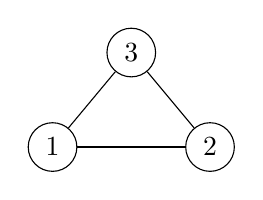
\begin{tikzpicture}
                \begin{scope}[
                        every node/.style={circle, draw},
                    ]

                    \node (1) at (0,0) {1};
                    \node (2) at (2,0) {2};
                    \node (3) at (1,1.2) {3};

                    \path (1) edge (2);
                    \path (3) edge (2);
                    \path (3) edge (1);
                \end{scope}
            \end{tikzpicture}
        \end{minipage}
        \begin{minipage}{0.3\textwidth}
            % \captionof{figure}{A graph with the spanning tree in black and arc subset $S$ in orange}
            with $\det \begin{pNiceMatrix}
                    1 & 0 & 1 \\
                    1 & 1 & 0 \\
                    0 & 1 & 1
                \end{pNiceMatrix} = 2$
        \end{minipage}
    \end{minipage}
\end{remark}
\begin{definition}
    A 0-1-matrix $A$ has the \vocab{consecutive ones-property} if the $1$'s in each row
    do not have any $0$'s between them, i.e. $0001111100$.
\end{definition}
\begin{corollary} \label{thm:cop-is-tu}
    A matrix $A$ with consecutive ones-property is totally unimodular.
\end{corollary}
\begin{proof}
    Suppose $T$ is a line of connected nodes.
    For each row, construct an arc from the first $1$ to the last $1$. Then $A$ is a network matrix for this graph.
\end{proof}
Note that there are totally unimodular matrices that aren't network matrices.
Furthermore, it's also possible to combine totally unimodular matrices to get new ones.
\begin{theorem}
    Let $A_1,A_2$ be two totally unimodular matrices. Then
    \[
        \left(
        \begin{BMAT}(rc){c|c}{c|c}
                A_1 & 0\\
                0 & A_2
            \end{BMAT}
        \right)
    \]
    is also totally unimodular. \label{thm:comp-unimod}
\end{theorem}
\begin{theorem}[Seymour]
    The set of totally unimodular matrices is fully defined by
    \begin{itemize}
        \item all network matrices,
        \item two additional $5\times 5$ matrices, and
        \item three different composition operations, e.g. \autoref{thm:comp-unimod}.
    \end{itemize}
\end{theorem}
\begin{conclusion}
    Network problems are the easiest $\IP$s.
\end{conclusion}